\newpage
\section{Operating Composite State}

\subsection{Mathematical Representation}

\noindent As \textit{Operating} is a composite state, it is defined as the tuple $S = (Q, \Sigma_1, \Sigma_2, q_0, V, \Lambda)$, where\\

\noindent $Q = \{Idle, Active, \textit{Stand-By}, Servicing\}$\\
\noindent $\Sigma_1 = \{press~finish, receive~start~signal, receive~service~signal, machine~fixed, power~out, power~back~on, \\
\indent cancel, completion\}$\\
\noindent $\Sigma_2 = \emptyset$\\
\noindent $q_0: Idle$\\
\noindent $V: \emptyset$\\
\noindent $\Lambda$: Transition specifications\\
\indent 1. $\rightarrow Idle$\\
\indent 2. $Idle \xrightarrow {\text {press finish}} Exit$\\
\indent 3. $Idle \xrightarrow {\text {receive service signal}} Servicing$\\
\indent 4. $Idle \xrightarrow {\text {receive start signal}} Active$\\
\indent 5. $Servicing \xrightarrow {\text {machine fixed}} Idle$\\
\indent 6. $Active \xrightarrow {\text {power out}} \textit{Stand-by}$\\
\indent 7. $Active \xrightarrow {\text {cancel}} Idle$\\
\indent 8. $Active \xrightarrow {\text {completion}} Idle$\\
\indent 9. $\textit{Stand-by} \xrightarrow {\text {power back on}} Active$\\

\noindent The UML state diagram is shown in Figure~\ref{fig:operating}.

\newpage

\subsection{State transition diagram}

\begin{figure}[h!]
	\centering
		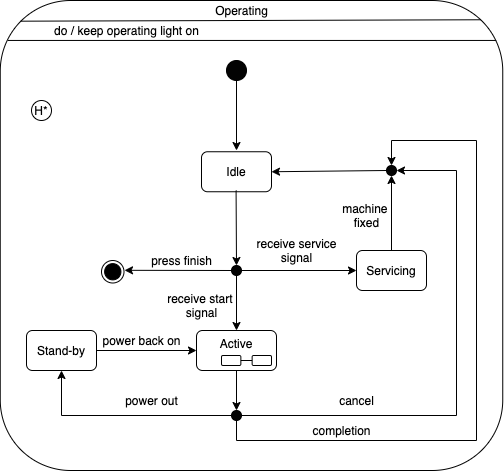
\includegraphics[width=0.8\textwidth]{Operating}
		  \caption{Operating State Diagram}
  \label{fig:operating}
\end{figure}
